\documentclass[a4paper]{article}

\usepackage[italian]{babel}
\usepackage[utf8]{inputenc}
\usepackage[T1]{fontenc}
\usepackage{microtype}
\usepackage{xcolor}
\usepackage{titlesec}
\usepackage{xargs}
\usepackage{multicol}

\usepackage{graphicx}

\usepackage[colorlinks]{hyperref}
\definecolor{RoyalBlue}{rgb}{0.0, 0.14, 0.4}
\hypersetup{
     colorlinks=true,
     linkcolor=blue,
     filecolor=blue,
     citecolor = black,
     urlcolor=cyan,}

\title{Algoritmo dei K-Nearest Neighbours}
\date{31 marzo 2021}
\author{Davide Peccioli}

\begin{document}
\maketitle

Dato un punto, per mezzo di questo algoritmo è possibile classificarli, associandovi una classe di appartenenza.

Il codice presentato, consente, dato un insieme di punti di cui si conosce la classe, ed un insieme di punti da testare, ma di cui comunque si conosce la classe, di stabilire per quali valori $k$ l'algoritmo funziona meglio.

\section{Funzionamento dell'algorimo}

L'algoritmo funziona sulla base di un insieme di punti di partenza (denominato \textbf{train set}), ciascuno associato alla propria classe: dato un punto da analizzare (denominato \textbf{A}), il risultato sarà la classe di appartenenza del punto stesso.

All'algoritmo viene passato un parametro $k$. Verranno presi i $k$ punti del \textbf{train set} più vicini ad \textbf{A}, e la classe più frequente tra questi punti sarò la classe assegnata ad \textbf{A} stesso.

\section{Codice}

Come già detto, il codice presentato non è semplicemente lo svolgimento dell'algoritmo, bensì un codice che permette di stabilire per quale parametro $k$ l'algoritmo funziona meglio sui punti considerati.

Il \href{https://github.com/DavideP02/Octave_KNN_Peccioli5H/blob/main/KNN.m}{codice commentato} è visualizzabile su GitHub.

\section{Risultati}

L'esecuzione su terminale del codice presentato è disponibile \href{https://youtu.be/Dq0btd1xUEI}{qui}.

I due grafici che sono stati prodotti dal codice sono:
\begin{figure}
\centering
\label{fig:punti}
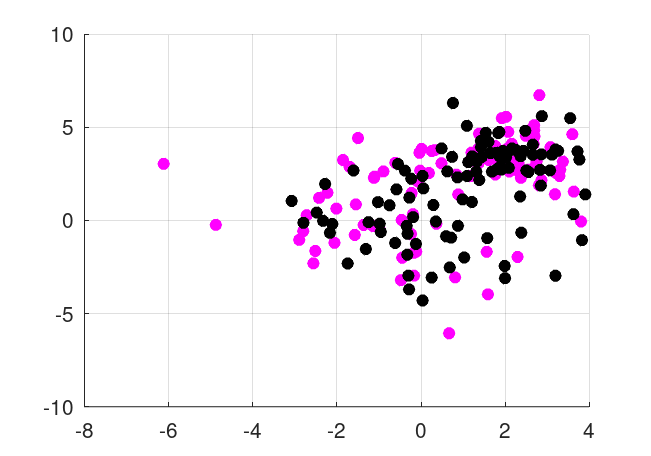
\includegraphics[width=10cm]{punti}
\caption{Punti di train e di test}
\end{figure}
\begin{figure}
\centering
\label{fig:acc}
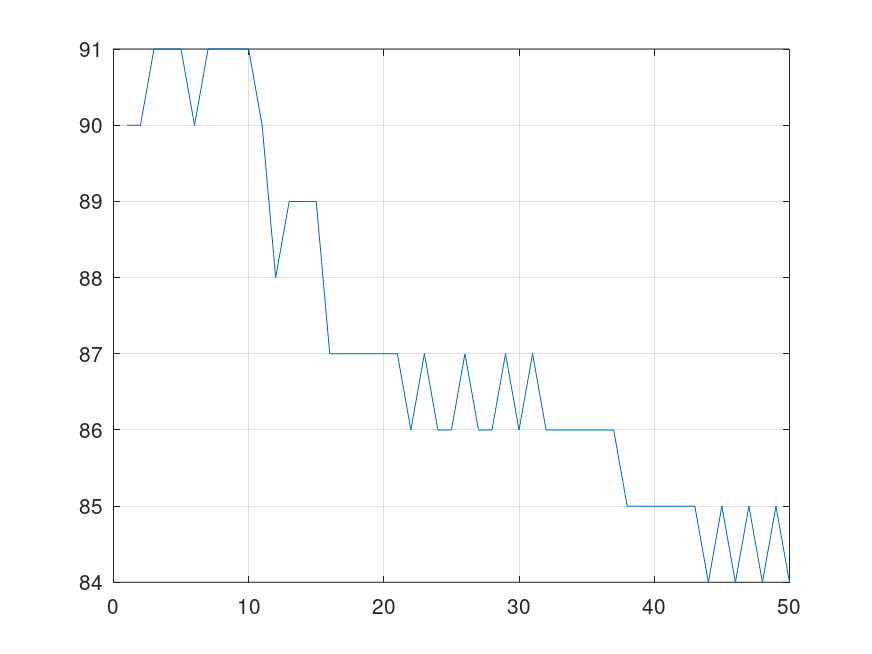
\includegraphics[width=12cm]{accuratezza}
\caption{Accuratezza al variare di $k$}
\end{figure}

Nella figura~\ref{fig:punti} possiamo vedere in nero i punti del \textbf{train set}, e in magenta i punti che verranno processati dall'algoritmo.

Nella figura~\ref{fig:acc} è rappresentato l'andamento dell'accuratezza (in percentuale) dell'algoritmo al variare di $k$, per valori da $0$ a $50$. Possiamo notare come contrariamente da quello che ci si può aspettare, i valori di $k$ per cui l'accuratezza è massima sono relativamente bassi:
\[
k \in K = \{3; 4; 5; 7; 8; 9; 10\}
\]

Per tutti i valori di $k\in K$ l'accuratezza è pari al 91\%, mentre il valore minimo, toccato con $k=100$ (non mostrato in figura) è del 50\%.

Con una piccola modifica al codice, è possibile stampare i punti dell'insieme di test per cui l'algoritmo (con $k=4$) non ha funzionato: il risultato è mostrato nella figura~\ref{fig:sb} (punti in rosso).

Possiamo quindi notare come l'algoritmo abbia fallito in una zona sul piano particolarmente densa di punti, e in cui quindi, probabilmente, la precisione dell'algoritmo non è sufficiente.

\begin{figure}
\centering
\label{fig:sb}
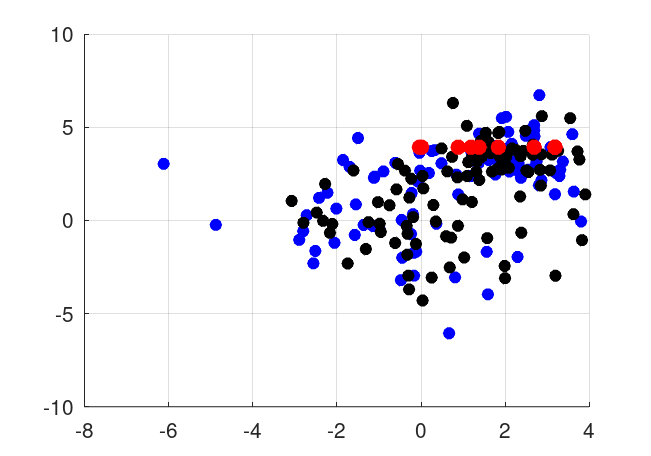
\includegraphics[width=10cm]{puntisb}
\caption{Punti di train e di test}
\end{figure}

\end{document}